%\documentclass[prb,preprint,showpacs,superbib]{revtex4}

\documentclass[prl,twocolumn,showpacs,twocolumngrid,superbib]{revtex4}


\usepackage{graphicx}
\usepackage{amsfonts}
\usepackage{amsmath}
\usepackage{bm}
\usepackage{alltt}
\usepackage{fancyhdr}
\newcommand{\bms}[1]{{\boldsymbol #1}}
\renewcommand{\thefootnote}{\fnsymbol{footnote}}

%\draft
%\tighten
\pagestyle{fancy}

\begin{document}

%%\title{Geometry Optimization for Dummys {\tt ;)} \footnotemark[1]} 
%%\title{A Simple Approach to Internal Coordinate Geometry Optimization\footnotemark[1]}
\title{Linear Scaling Geometry Optimization via the Quasi- \\ 
       Independent Curvilinear Coordinate Approximation\footnotemark[1]}
%\title{A New Look at Geometry Optimization: The Quasi- \\ 
%       Independent Curvilinear Coordinate Approximation\footnotemark[1]}
%%\title{A New Look at Geometry Optimization; the Quasi Independent Curvilinear Coordinate Approximation\footnotemark[1]}

\author{K\'aroly N\'emeth\footnotemark[2]}
\author{Matt Challacombe}

\affiliation{Theoretical Division,\\ Los Alamos National Laboratory, \\ Los Alamos, NM 87545, USA}

\date{\today}

\begin{abstract}
{
This article presents a new and efficient alternative to well established
algorithms for molecular geometry optimization.   The new approach 
exploits the approximate decoupling of 
molecular motions
% energy gradients 
in a curvilinear 
internal coordinate system,  allowing separation  of the 3$N$-dimensional
optimization problem into an ${\cal{O}}(N)$ set of quasi non-interacting
one-dimensional problems.  Each  uncoupled optimization is developed by fitting 
energy gradients in the internal coordinate system followed by root finding.  
This new approach is competitive with the best geometry optimization algorithms 
in the literature, achieves superlinear convergence and works well for large 
biological problems with complicated hydrogen bond networks and ligand binding 
motifs.}

\smallskip
\noindent{\bf Keywords}: 
geometry optimization, linear scaling, 
curvilinear internal coordinates, fitting
\end{abstract}

\maketitle

\footnotetext[1]{LA-UR-04-1097}
\footnotetext[2]{\tt KNemeth@LANL.Gov}

\section{Introduction}

Recently, $N$-scaling electronic structure algorithms ($N$ is the system size)  have 
realized their promise, delivering energies and forces on nuclei for large systems at 
both a numerical accuracy and theoretical level suitable to begin addressing many complex 
problems.  For example, it is now possible to routinely apply hybrid Hartree-Fock/Density 
Functional theory to fragment models in molecular biophysics involving complicated 
networks of hydrogen bonds and metal-ligand binding motifs and several hundred atoms using basis sets of triple-zeta plus 
polarization quality.  However, despite favorable scaling properties, ${\cal O}(N)$ 
methods typically carry a larger cost prefactor than their conventional counterparts.  Thus, 
in addition to parallelism, developing efficient algorithms to drive the core engines of 
linear scaling electronic structure theory is paramount.  Of these, perhaps the most useful 
driver of electronic structure theory is the molecular geometry optimizer, which follows 
the energy gradient downhill to a local minimum.   

This paper presents a new concept for the optimization of molecular geometries based on
the approximate separability of 
molecular motions
%energy gradients 
in curvilinear internal coordinate 
systems, and the recent availability of fast transformations to and from these coordinate systems 
for large molecules \cite{paizs_coordtrf1,nemeth_coordtrf1,paizs_coordtrf2,nemeth_coordtrf2}.  
Internal coordinates represent the internal motions of a molecule and can 
be described well in terms of bond stretches, angle bendings and dihedral torsions.
%Internal coordinates are normal mode-like degrees of freedom that include bond stretches, angle bendings, 
%dihedral torsions and  out of plane bendings.  
These different motions, which are related to chemical concepts, lead to
an approximate energy and length scale separation, which is manifested
in a strong diagonal dominance in the matrices of second and higher order
energy derivatives.
%Energy scale differences characteristic of these different motions lead to 
%a strong diagonal dominance of the matrix of energy second derivatives 
%(the Hessian) as well as higher order anharmonic energy tensors;  
%off diagonal elements of the 
Off diagonal elements of the 
internal coordinate Hessian are typically an order of magnitude smaller than the diagonal ones
\cite{pulay_69,fogarasi_diaghess,Pulay_natural_internals,pulay_review,pulay_dynamics}.
This is the basis for an approximate decoupling of molecular motions in terms of internal coordinates.

An observation central to 
the present
%this 
contribution is that internal coordinate gradients show recognizable trends 
during optimization, and these trends can be captured by curve fitting and used to predict minima by 
one-dimensional extrapolation.  This is illustrated in Fig.~\ref{NH3outp6}, showing a typical progression of 
internal coordinate gradients.  We therefore propose solving the molecular geometry optimization problem as 
an $N_{\rm int}$ 
dimensional
set of uncoupled one-dimensional equations, where $N_{\rm int} \propto N_{\rm atoms}$ is 
the number of internal coordinates. 

\begin{figure}[h]
\resizebox*{3.5in}{!}{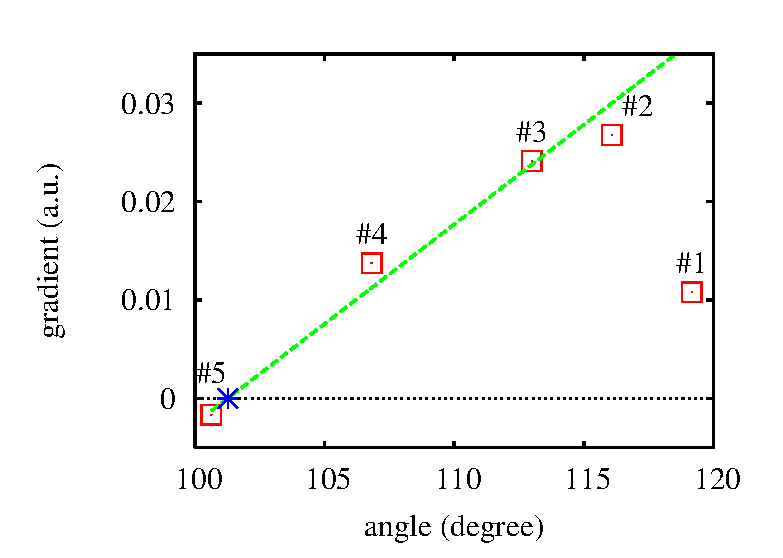
\includegraphics{picture1_2.eps}}
\caption{
Progression of gradients on a valence angle bending coordinate of
ammonia. Energies and forces were obtained by the PBE 
density functional model in STO-3G basis set.
The optimization was started from near planar geometry, i.e.
from the vicinity of a transition state, and converged to a local 
minimum of the potential energy surface. The numbers in the picture
indicate the sequence of optimization steps. The dashed line represents
a linear fit, the star the predicted location of the minimum.}
\label{NH3outp6}
\end{figure}

\subsection{Conventional Methods}

Over the last three decades, internal coordinate geometry optimizers have become the standard 
tools for 
finding
%locating 
local minima when energies and forces are calculated by electronic structure 
theory \cite{10papers}. Internal coordinates describe the internal motions of molecules 
with chemical degrees of freedom such as bond-stretches, valence angle bendings and the torsions 
of dihedral angles. These curvilinear coordinates are constructed from non-linear functions of the 
Cartesian coordinates of atomic nuclei \cite{wilson}.

The reduced 
vibrational
%energetic  
coupling achieved with internal coordinates provides an advantage 
in molecular geometry optimization \cite{pulay_review} and molecular dynamics \cite{pulay_dynamics}.
Thus, a full Newton step in Cartesian coordinates will typically generate much more harmonic and anharmonic coupling effect
than a full Newton step carried out in internal coordinates.
%Thus, a full Newton step in Cartesian coordinates will typically generate much higher order 
%anharmonic coupling relative to a full Newton step carried out in internal coordinates.
An excellent discussion of this issue can be found in the Introduction of Ref.~\cite{Pulay_natural_internals}.

Today, the most aggressive internal coordinate algorithms have been highly optimized for 
small molecule quantum chemistry.  These methods typically generate a Cartesian Hessian,
either exactly or approximately. This Cartesian Hessian is then transformed into an internal 
coordinate representation, and an internal coordinate Newton step is taken. The internal 
coordinate step is then transformed back to a Cartesian displacement and used to increment the 
molecular geometry.

There are many variations on this approach.  
Cartesian Hessians are usually calculated by updating algorithms
in the framework of the quasi-Newton approach \cite{RFletcher}.
A fequently used updating scheme is the Broyden-Fletcher-Goldfarb-Shanno (BFGS) technique \cite{RFletcher}. 
These methods provide an approximate Cartesian Hessian and avoid
computing the exact Hessian.
%For example, updating schemes related 
%to the Broyden-Fletcher-Goldfarb-Shanno (BFGS) technique \cite{RFletcher} may be used 
%to avoid computing the exact Cartesian Hessian.
%\cite{}. [citation of Fletcher's book account on this]
With increasing system size, storing,
transforming and potentially inverting the full Hessian matrix becomes expensive and it becomes
favorable to consider diagonal or semi-diagonal approximations to the internal coordinate Hessian. 
This severely truncated Newton or  ``force relaxation'' method typically obtains diagonal values 
{\em a priori} from spectroscopic data or empirical force-fields 
\cite{pulay_69,pulay_review,sellers,fogarasi_diaghess,Pulay_natural_internals,van_alsenoy_98,lindh}.
It is worth noting that the landmark RHF/4-21G optimization of Crambin by Van Alsenoy \cite{van_alsenoy_98}
was carried out in just 79 steps using the force relaxation approach of Sellers \cite{sellers}.
In these 
%some !!! in all algorithms !!!
algorithms, strong damping \cite{sellers} or line searching \cite{sclegel_linesearch}
is required to avoid divergence. 
Another important technique to control and accelerate convergence of geometry optimization 
is the geometric DIIS \cite{Pulay_GDIIS} (GDIIS). While geometric DIIS is a simple technique, 
its successful application may require many intricate modifications \cite{Farkas_GDIIS}.  A recent 
review and comparison of these algorithms and their technical details can be found in Ref.~\cite{bakken}.  

\section{A New Concept}

In the Newton-Raphson method, the correction to the Cartesian vector $\bf x$ of nuclear positions 
is $\delta {\bf x}  = - {\bf g}\cdot {\bf h}^{-1}$,  where $\bf h$ is the Hessian, a matrix of 
energy second derivatives with respect to nuclear displacement.  Thus, a step along a specific 
element of $\bf x$ is coupled to all components of $\bf g$ through off-diagonal elements of $\bf h$.  
Alternatively, it is possible to work in the principal axis system of $\bf h$, or normal modes, 
which are uncoupled to second order as the Hessian is diagonal in this representation. 

Consider now a Newton scheme on an ideal harmonic surface.
The normal modes remain uncoupled as the optimization proceeds.
The diagonal Hessian elements can now be calculated by
numerical differentiation of the gradients 
for each normal mode, as soon as 
the gradients are available at least at two different values
of each normal mode. 

There is a conceptual alternative of this numerical
differentiation, which allows for generalized applications, when
surfaces are anharmonic and normal modes are not available. 

First, one has to see, that the numerical differentiation of the
gradients and the Newton step along each normal mode
is equivalent to a one-dimensional line-fit and root 
finding.
The root of the fitted line is the location of the 
minimum along the normal coordinate considered.

Now, we can make use of the observation, that internal coordinates
are well decoupled both on harmonic and
anharmonic levels of the potential energy surfaces. In fact,
internal coordinates are more advantageous in the
treatment of anharmonicities then normal modes \cite{fogarasi_diaghess}.

The fitting of gradient curves can thus proceed over internal coordinates,
with the observation, that no perfect line fits can be expected.
This is due to the effect of harmonic and anharmonic couplings,
which scatter the gradients along a pattern, typically along a line.

A simple line fit to the gradients for each internal coordinate
reflects the expectation, that close enough to the minimum
the surface should be harmonic and the gradient curves are linear.
Of course, one can consider higher order fits, with the intention
of accumulating more explicite anharmonic effects. However, the
stability of such a scheme does not seem to be easily achievable.
While the simple line fit is stable, robust and provides smoothing
of noisy data, higher order fits are much less stable, and provide
less smoothing effects, at least in the phase of optimization, when
large geometry corrections happen.

The reason, why the fitting scheme should work is the effective
decoupling of internal coordinates, which has been demonstrated
by the success of force relaxation methods \cite{pulay_review,sellers,van_alsenoy_98}. We call the concept of not applying any explicite vibrational 
coupling in geometry optimization
the Independent Curvilinear Coordinate Approximation. 

Data points of the gradient curve can be weighted. Our observation is,
that an appropriate weighting scheme greatly improves the efficiency
of the optimization process. As described later in this paper, 
the weights should reflect local coupling effects. Since such a weighting
scheme gives an implicite account of the most important coupling effects, we
name our approach 
``QUasi Independent Curvilinear Coordinate Approximation'' or QUICCA.

%Consider now an approximate second order scheme, where the normal coordinates remain 
%diagonalizing (at least for a few geometry steps).  
%In this case, gradient information may 
%be used to construct a finite difference approximation to the diagonal Hessian elements at 
%each new geometry.  After a number of steps, the finite difference approximation may be 
%replaced in favor of a curve fit of the gradient data, which may yield higher order 
%accuracy for large displacements.  A little more thought, and the possibility of accumulating 
%anharmonic information through additional terms in the fitting polynomial presents itself.  
%Of course, as the optimization proceeds, the normal coordinates corresponding to the
%initial structure will not remain diagonalizing and coupling effects will manifest, leading to 
%noise in the gradient data.  

%Adopting instead an internal coordinate system, the concept developed so far is an Independent 
%Curvilinear Coordinate Approximation similar to force relaxation methods \cite{pulay_review,sellers}, but 
%with a constantly updated  curve fit that replaces the need for static diagonal elements of the Hessian.
%This approach works well, but coupling effects can lead to noise in the gradient data, making 
%the standard least squares curve fit unreliable.  However, a significant advance can be
%realized by instead using a weighted curve fit, with the weights depending {\em implicitly}
%on coupling effects.   This is the new concept behind our approach to optimization that we 
%call the ``QUasi Independent Curvilinear Coordinate Approximation'' or QUICCA. 

Explicitly then, application of QUICCA to geometry optimization involves the  projection of Cartesian 
gradient information onto an 
%uncoupled !!! "internal coordinate" means inherently "uncoupled"  
$N_{\rm int}$ dimensional internal coordinate space.  Energy gradients 
are accumulated for each internal coordinate, as shown in Fig.~\ref{NH3outp6}, and used to formulate 
$N_{\rm int}$ independent curves by weighted least squares.  At each step, these curves are extrapolated 
(or interpolated) to zero, with collective changes in the internal coordinate system taken as an approximate 
minimum for the system as a whole. The final back-transformation of the step to Cartesian coordinates merges 
these displacements, reconciling any redundancies in the internal coordinate system. The quality of this 
collective extrapolation is determined by severity of 
the independent curvilinear coordinate approach,
%the low order coupling, 
redundancy of the internal 
coordinate system and the accuracy of the fit.  The QUICCA approach to geometry optimization is simple to 
implement and scales linearly with system size.  It overcomes low order coupling effects through averaging and 
weighting of the curve fit and also admits the accumulation of anharmonic information.  

From the methodological point of view, QUICCA represents two new developments.
One is the generalization of numerical differentiation by the use of a line fit, that
allows the elimination of the empirism present in force-relaxation methods. The
line fit also allowes to replace the Newton step by one-dimensional root-finding.
The other new contribution is, that QUICCA is capable to take an implicite 
account of local couplings via a weighted least squares fit.

\section{Implementation}

\subsection{Recognition of Internal Coordinates} \label{recognition}

The present implementation of QUICCA employs a redundant set of primitive internal 
coordinates. Similar coordinate systems are used by a majority of other internal coordinate optimizers 
\cite{bakerstest,eckert,Pulay_natural_internals,fogarasi_diaghess,schlegel_on2iter}.  
The generation of these coordinates starts with the recognition of of covalent bonds, 
based on atomic Slater radii \cite{SlaterRad}  multiplied by an empirical factor of 1.3. 
Weak bonds are recognized on the basis of atomic van der Waals (VDW) radii \cite{JMOLtable}.
Note, that no VDW contact is allowed between atoms, which are second or third neighbors in the 
covalent bonding scheme.  The search for neighboring atoms is carried out by dividing 
the system into small cubes a few angstroms on a side, and bonds are looked for only within 
each box and between nearest neighbor boxes.  This divide-and-conquer scheme ensures the fast 
and linear scaling recognition of bonding for large molecules. The bonding scheme is then 
stored in a sparse topology matrix.

At each step of the optimization the actual bonding scheme is determined and the corresponding 
sparse topology matrix is stored on disk.  Then, topology matrices of the most recent steps are 
summed up to result in a merged topology matrix.  The number of merged matrices is always equivalent 
to the number of remembered steps, $n_{\rm fit}$, employed by the curve fitting. In the current implementation 
$n_{\rm fit}=7$, but it can be much larger or smaller.  The merged topology matrix reflects the possibility of 
bond-formation and bond vanishing during the optimization of large molecules.  Formation of a new 
bond can often happen due to hydrogen bond formation. Bond vanishing can happen when, for example,
a van der Waals contact becomes large.  This provides a merged, consistent internal coordinate 
system from step to step.  It is important to use internal coordinates
of the merged bonding scheme later, when the $n_{\rm fit}$ Cartesian gradient
vectors are transformed into internal coordinate representation. The use of the merged bonding 
scheme insures the convergence of the coordinate transformation for each of the remembered steps.
Inclusion of coordinates from the remembered steps only minimally increases the number of internal 
coordinates and the redundancy of the coordinate set, as the final merged topology matrix is 
determined directly from primary topology matrices rather than the merged ones at previous cycles.

Based on the topology matrix of the merged bonding network, all other primitive 
internal coordinates, such as bond angles, torsions, linear bendings and 
out-of-planes are recognized. Torsions are selected so that each bond will be 
associated with only a single torsional coordinate.

\subsection{Preparing the Data}

Cartesian coordinates and the corresponding Cartesian gradients of the $n_{\rm fit}=7$ 
most recent geometries are read from disk. Based on the most recent definition of the 
bonding scheme they are transformed into the internal coordinate representation,
determined by the merged bonding scheme.
The coordinate transformation is carried out as described in Ref.~\cite{nemeth_coordtrf1}, 
while the necessary intermediate sparse matrices of 
the coordinate transformation are re-generated. 
This is a very inexpensive step, due to the extreme sparsity of the vibrational B matrix \cite{wilson}. 
Thus the primary objects of the proposed geometry optimization,  the internal coordinates and their gradients,
are re-created at each step allowing on the fly redefinition of the 
coordinate system.

In order to avoid problems due to the periodicity of torsional angles, reference points are used, 
eg. the torsional angle values of the most recent geometry. Each torsional angle is set to its 
periodic equivalent closest to the reference point, by a shift of $\pm 2\pi$, while its gradient value does not change.

\subsection{The Weighted Curve Fit} \label{Sweights}

At this point,  we have a set of $n_{\rm fit}$ coordinate - gradient pairs for each individual 
internal coordinate, such as the one presented in Fig. \ref{NH3outp6}. These data 
pairs parametrize progression of the gradient during the $n_{\rm fit}$ most recent steps of the 
optimization.  This data is now used to fit curves for each of the $N_{\rm int}$ coordinates using the 
well established and robust {\sc SLATEC} routine {\sc POLFIT} and its dependencies \cite{slatec}, 
which allow a weighted least squares fit.

The choice of weight is a key factor in the behavior of the QUICCA algorithm, as it is used to prioritize 
reliable portions of the data and to generally smooth noisy trends.  
Originally, we considered the standard expression $w_{k}^{(i)}=\left(1/{g_{k}^{(i)}}\right)^2$ for the weight 
of the $k$-th internal coordinate at the $i$-th geometry, which is generally recommended for use in curve 
fitting \cite{numerical_recipies}.  These weights however do not 
account for the fact that the gradient of the $k$-th internal coordinate may be small, while 
its environment may contain large gradients indicating the possibility of large changes in the $k$-th 
internal coordinate due to coupling effects.  Thus, a data point with high environmental tension 
is less reliable than a point with neighboring coordinates that are relaxed.   
Local sums of the gradient squares,
\begin{equation}
\label{weights}
w_{k}^{(i)} = \left[ \sum_{l} g_{l}^{(i)} \frac{1}{|H_{ll}^{}|} g_{l}^{(i)} \right]^{-1} ,
\end{equation}
incorporate this effect, where  $l$ indexes internal coordinates that have atoms in common with 
the $k$-th internal coordinate, and $H_{ll}^{}$ is an approximate Hessian.  The terms 
$H_{ll}^{}$ yield dimensionally correct sums, since each of the gradient components  $g_{l}$ has a 
different measure for stretches than for bendings or torsions.  

For each coordinate $k$, the sum over $l$ is determined by the topology matrix, given by the symbolic 
structure (graph) of the sparse matrix $G_{i}=BB^{t}$, which obtains from the sparse Wilson's $B$ 
matrix \cite{wilson}.  We have considered more delocalized interactions as well, such as those deriving 
from the graph of $G_i^2$, but they did not provide any significant improvement in test calculations.

Values of $1.0$ a.u. for stretches, $0.1$ a.u. for bendings, linear bendings and out-of-planes and $0.01$ a.u.
for torsions are used as an 
initial guess for the $H_{ll}$. Note, that only the relative values of $H_{ll}$
are important for the fitting process, as the fitting parameters are determined
by the relative values of the weights. Our $H_{ll}$ values are similar to those used to provide 
an initial guess for the Hessian in variable metric algorithms \cite{bakken}.  
The choice of the relative values of $H_{ll}$ provides on opportunity to scale
the relative weights of rigid and floppy coordinates and thus
promote the relative speed of convergence in favor of floppy coordinates.
However, in small molecule tests we have found only a small effect
due to this lengthscale-enhancement (see Section \ref{Sresults}).
It is possible to refine the initial values of $H_{ll}$ during the 
optimization, but we do not consider this point in the present work.

While it is possible to employ second and third order polynomials in the fit, extrapolation
to zero is most robust with just a line, and that is the approach we employ here.  We believe there
is opportunity for the development of higher order approximations,  but the construction of such 
schemes is beyond the scope of the present paper.  A primary difficulty in the construction of higher 
order fits is that distinguishing between noise and signal is more difficult.  Also, there are stability 
issues of extrapolation versus interpolation with higher order polynomials.

\subsection{Minimum or Transition State?}

Transition states are indicated by a gradient curve with  negative tangent at the position
of the root.  For example, in Fig. \ref{NH3outp6} the tangent of the gradient curve is negative 
in the vicinity of the planar structure (structure \#1). This is so, as the planar ammonia 
is a transition state. The tangent of the gradient curve thus offers a convenient tool 
to control convergence to either a minimum or transition state.  In the present article we 
restrict the discussion to avoiding transition states and finding local minima. 
Whenever the local tangent of the gradient curve is negative, the optimizer employs a simple force relaxation step,
\begin{equation}
\label{tseq}
\varphi_{k}^{(i+1)} = \varphi_{k}^{(i)} -g_{k}^{(i)}/|H_{kk}^{(i)}| ,
\end{equation}
where $i$ denotes the serial number of the optimization step and $\varphi_{k}$ is the $k$-th internal coordinate.
This way those transition states that are well localized to a few internal coordinates
are avoided.  It is not clear how the present implementation would behave in the 
case of a more delocalized transition state, spanning many internal coordinates, which 
are in principle possible but rarely occur.  

Combined internal coordinates, such as the natural internals \cite{Pulay_natural_internals} or the
delocalized internals \cite{Baker_deloc_1}, hold the possibility of identifying delocalized transition 
states by gradient fitting.  An analysis by  Wales {\it et.al.} \cite{Wales_saddlepoint} provides 
insight into the numerical problems involved in controlling convergence to a minimum without an 
accurate Hessian.  Note that, even with a good quality Hessian update, such as BFGS \cite{RFletcher},
there is no guarantee to converge into a minimum instead of a transition state. 
This is because positive definiteness of an approximate Hessian does not guarantee
the positive definiteness of the exact Hessian.  Thus, the exact Hessian remains the only 
certain metric for determining the character of extremal points in the potential energy 
surface \cite{Pulay_natural_internals}.

\subsection{Initial steps}

In the very first step of the optimization, a force relaxation step is used with the usual 
diagonal Hessian estimates of 0.5 a.u. for stretchings, 0.2 a.u. for bendings and 0.1 a.u.for 
torsions.  This initial step is equivalent with the one traditional optimizers use.

\subsection{Step size control and backtracking}

Experience with QUICCA has shown that extrapolations larger 
than the range spanned by the fitted data points are unreliable.   Thus, 
while QUICCA  always tries to achieve the predicted minimum, 
stepsize control is imposed, limiting the step  by  the fit range or to 
0.3 au, whichever is less.   This maximum allowed value of the stepsize, 0.3 au, 
is similar to that used by other optimizers \cite{eckert}.  

The range spanned by the fitted data is in some sense an uncertainty.  
Refining and formalizing quantification of this uncertainty is another area of 
opportunity for improvement of the QUICCA optimizer, which is beyond the 
scope of this article.  We note however, that it might be more effective
to use a filtered range of the data points, based on their weights. 
For example, compute the range including only those points with weights that 
comprise, say,  99.99 percent of the total.   Alternatively, statistical 
tests could be employed to filter out outlying points.  We note that issues of
uncertainty in stepsize control are certain to be far more complex for higher 
order fits, and advanced statistical methods may have a significant role 
to play in this area of development.

\subsection{Backtracking}

While the above stepsize control is designed to avoid potential instabilities,
it is still possible to take steps that will increase the total energy.  In 
this case, there are a number of options.  We can live with the increase, 
hoping it will nevertheless improve the information content used to build the energy 
surface.  We can backtrack, uniformly reducing the step, typically by half, and re-evaluate
the energy to see if it decreases.   Alternatively, we can employ a more 
sophisticated and expensive line search to determine a minimizing step.  

There are many ways to carry out a line-search.  Perhaps the most widely employed 
approach is the endpoint algorithm of Schlegel \cite{sclegel_linesearch}.  This algorithm
employs energies and gradients at the endpoints to yield a quartic interpolant.  This
approach will work well if the interpolant varies smoothly between endpoints.  We have
implemented this approach to the line-search, but found that it does not perform 
reliably, especially when large steps are made.   It may be that midpoint algorithms
are more appropriate, but we have not explored this further.

Our experience with QUICCA is that simple back-tracking is both cheaper and more effective
than the endpoint line-search.  During back-tracking, a  bad step is recognized by an elevated
energy before any gradient evaluation takes place. Then, the step-size is halved,
and a new energy is calculated.  This process is repeated until the energy becomes lower,
typically requiring just one halving.

\subsection{Iterative back-transformation}\label{transformation}

Once predictions of internal coordinate displacements are made, they are passed to the 
iterative back-transformation to generate a new set of Cartesian coordinates, as in 
Ref.~\cite{pulay_review}.   However, there is no guarantee that there exists a set of 
Cartesian coordinates that can exactly realize the new, predicted internal coordinates.  
For example, a prediction of angles in a triangular molecule can sum 
to a value greater than or less than 180 degrees. Such conflicts are a consequence of 
the redundant internal coordinate system.  

Displacements
%Elements 
of the updated internal coordinate system that result in geometric conflicts 
will be projected out during the iterative back-transformation. However, if 
these conflicts are too large, the iterative back-transformation may fail to converge,
or it may produce a set of Cartesian coordinates that violates the predicted internal 
coordinate values. Typically, these violations are larger, when large steps are
taken and become smaller close to convergence.
%  Typically, such violations are small, but can  lead to minor problems 
%when using very tight convergence criteria.

%One approach to avoiding this problem is to work with linear-combinations of primitive internal
Our preferred approach to avoiding this problem is to work with linear-combinations of primitive internal
coordinates, such as the natural \cite{Pulay_natural_internals} or delocalized
\cite{Baker_deloc_1} internal coordinates, which minimize geometric conflicts.  
Another cure for redundancies is to apply a projection technique prior to the iterative-back 
transformation \cite{pulay_review}, which can eliminate problems to first-order, but does not 
guarantee convergence for large steps.

In our present implementation, geometric conflicts are dealt with solely by the iterative back-transformation.
In the case of non-convergent back-transformation,  our algorithm will attempt the back-transformation
again, but with the original internal coordinate displacements halved.  If the repeated transformation 
also fails, it usually indicates an incomplete set
of internal coordinates 
and the program stops.  An incomplete 
set can also scuttle convergence of the Cartesian to internal gradient transformation \cite{nemeth_coordtrf1}. 
Note, that an appropriate internal coordinate recognition program 
together with suitable internal coordinate step-size control
can always avoid non-convergent back-transformation.

\subsection{Realization}

The QUICCA geometry optimization algorithm has been implemented in the
object oriented FORTRAN-90/95 programming language and is part of
the MondoSCF suite of linear scaling quantum chemistry codes \cite{MondoSCF}.
It has been successfully tested on different platforms, compilers and operating
systems. 

\subsection{Scaling}

At each geometry step, the cost of QUICCA is associated only with 
recognition of internal coordinates, the coordinate 
transformations and the fitting process. The recognition of internal 
coordinates scales linearly, as described in Section \ref{recognition}.  
The effort spent on fitting is 
$ {\cal O}(N_{\rm int})$ with $N_{\rm int} \propto N_{\rm atoms}$, as the number of 
points employed by each fit is a constant.  Likewise, the coordinate transformations scale linearly with system 
size as pointed out in Ref.~\cite{nemeth_coordtrf1}.

\section{Results and Discussion} \label{Sresults}

\begin{table}[h]
%\squeezetable
\caption{
Number of geometry optimization steps to convergence of Baker's test set
(up to 30 atom molecules) for the QUICCA optimizer and also for other 
advanced 
%more well developed 
algorithms from the literature.  Calculations have 
been carried out at the RHF/STO-3G level of theory.  All of the reported
calculations used local primitive internal coordinates, except those
of Bakken {\it et.al.} who used extra redundant coordinates \cite{bakken}.
}
\label{Bakers_test}
\begin{tabular}{lccccc}
\toprule
Molecule               & QUICCA  & Bakken         & Eckert         & Lindh         &  Baker  \\
                       &         & {\it{et al.}}  & {\it{et al.}}  & {\it{et al.}} &    \\
                       &         &  \cite{bakken} &  \cite{eckert} & \cite{lindh}  &  \cite{bakerstest} \\
\colrule
Water                  &   4    &   4    &    4    &    4   &   6     \\
Ammonia                &   4    &   5    &    6    &    5   &   6     \\
Ethane                 &   4    &   3    &    4    &    4   &   5     \\
Acetylene              &   4    &   4    &    6    &    5   &   6     \\
Allene                 &   3    &   4    &    4    &    5   &   5     \\
Hydroxysulphane        &   8    &   7    &    7    &    8   &   8     \\
Benzene                &   2    &   3    &    3    &    3   &   4     \\
Methylamine            &   4    &   4    &    5    &    5   &   6     \\
Ethanol                &   5    &   4    &    5    &    5   &   6     \\
Acetone                &   4    &   4    &    5    &    5   &   6     \\
Disilyl ether          &   9    &   8    &    9    &   11   &   8     \\
1,3,5-trisilacycl.     &   5    &   9    &    6    &    8   &   8     \\
Benzaldehyde           &   5    &   4    &    5    &    5   &   6     \\
1,3-difluorobenz.      &   4    &   4    &    5    &    5   &   5     \\
1,3,5-trifluorob.      &   3    &   4    &    4    &    4   &   5     \\
Neopentane             &   5    &   4    &    4    &    5   &   5     \\
Furan                  &   6    &   5    &    6    &    7   &   8     \\
Naphtalene             &   6    &   5    &    6    &    6   &   5     \\
1,5-difluoronapht.     &   6    &   5    &    6    &    6   &   6     \\
2-hydroxibicyclop.     &   7    &   9    &    9    &   10   &  15     \\
ACHTAR10               &  10    &   8    &    9    &    8   &  12     \\
ACANIL01               &  11    &   7    &    8    &    8   &   8     \\
Benzidine              &   8    &   9    &    7    &   10   &   9     \\
Pterin                 &  12    &   8    &    9    &    9   &  10     \\
Difuropirazine         &   6    &   6    &    7    &    7   &   9     \\
Mesityl oxide          &   5    &   5    &    6    &    6   &   7     \\
Histidine              &  11    &  16    &   14    &   20   &  19     \\
Dimethylpenthane       &   6    &   9    &   10    &   10   &  12     \\
Caffeine               &   7    &   6    &    7    &    7   &  12     \\
Menthone               &  13    &  12    &   10    &   14   &  13     \\
\colrule
Total                  & 187    & 185    &  196    &  215   & 240     \\
\botrule
\end{tabular}
\end{table}

\subsection{Baker's test set}

The performance of the QUICCA optimizer has been tested on Baker's suite \cite{bakerstest} of 
small test molecules, and is listed in Table~\ref{Bakers_test}, along with values from more traditional 
algorithms.  At convergence, the magnitude of the maximum Cartesian force vector is required to be less 
than $3\times10^{-4}$ au for each atom.  This criterion is tighter than that employed in other studies 
Ref. \cite{bakerstest}, which require only that the maximum Cartesian force component (X, Y or Z) be less 
than $3\times10^{-4}$ au.  In addition to this criterion,  an absolute energy change less than 
$1\times10^{-6}$ au or a predicted internal coordinate displacement less than $3\times10^{-4}$ au at the last 
geometry is required.  The energies of the optimized structures have been reproduced to all digits given 
in Ref.~\cite{bakerstest}. 

The current implementation of QUICCA, achieving a total of 187 geometry steps for Baker's test suite, is 
competitive with Bakken's algorithm, requiring 185.  

Bakken's method \cite{bakken} appears to be the current 
optimal selection of techniques
for Hessian-update based internal coordinate methods. It is based
on the BFGS update \cite{RFletcher}, the Rational Function Optimization
scheme \cite{benerji_RFO} and a Newton trust-region model \cite{RFletcher}. An important addition
to these techniques is the application of
extra redundant coordinates, which contributes to the success of Bakken's
algorithm as compared to other traditional schemes. Extra redundant internal 
coordinates are local distance coordinates, which bridge the terminal atoms
of all valence angles and most of the dihedral angles.
%Based on a variable metric (quasi-Newton) 
%Cartesian Hessian, Bakken's method combines a number of well developed methods from the literature, 
%including a dynamic trust radius scheme,  an extra-redundant coordinate system, BFGS update of 
%the Hessian and the Rational Function method for quasi-Newton optimization.  

In contrast, the
current implementation of QUICCA employs the redundant primitive internal coordinate system, a weighted line
fit and simple backtracking.  

In two cases (ACANIL01 and Pterin), the QUICCA optimizer proved to be 
considerably slower 
than the best traditional techniques.   We believe these cases may be improved by introducing a
more sensitive weighting scheme, and/or employing a more sophisticated internal coordinate
system as discussed above in Section~\ref{transformation}.

Note that, these results have been achieved without the use of traditional convergence acceleration 
algorithms such as geometric DIIS (GDIIS) \cite{Pulay_GDIIS,Farkas_GDIIS}.  It is of course entirely 
possible to deploy the GDIIS algorithm together with QUICCA, but we leave this avenue open for future 
work.

Our experience shows, that relative large variations in the values of $H_{ll}$
as applied in the construction of weights (see Section \ref{Sweights})
do not cause big differences in the number of optimization steps on small
molecules. For example a set of $0.5$, $0.2$ and $0.1$ a.u. for $H_{ll}$ 
(instead of our standard, $1.0$, $0.1$ and $0.01$ a.u.)
results in 189 steps instead of 187 on Baker's test set.
The largest difference was present in Dimethylpenthane, which converges
2 steps faster when using the standard $H_{ll}$ values. 

In the Baker's test suite, about three force evaluations have been saved by 
using backtracking. Without the application of backtracking, Baker's test set
converges in 190 steps. 
This suggests that the core QUICCA algorithm is robust and
does not often overstep.  We can understand the stability achieved by the core QUICCA
algorithm by considering a hybrid force relaxation method, based on Eq.~\ref{tseq},
in which the diagonal Hessian elements $H_{ll}$ are obtained from the 
curve fit, but the uncoupled (truncated) Newton step is carried out with the {\em current} 
gradient.  We have tested this alternative, but it turned out to be oscillatory 
in many cases, requiring excessive backtracking.  This should be contrasted with the
full QUICCA algorithm, which uses root finding, and to first order is equivalent with 
an approximate Newton step taken with the {\em fitted} gradient.   Thus, the full 
QUICCA algorithm is successful not only because it generates up-to-date curvature information, 
but because it achieves stability through smoothing effects derived from the weighted fit.

%\begin{figure}[h]
%\resizebox*{3.5in}{!}{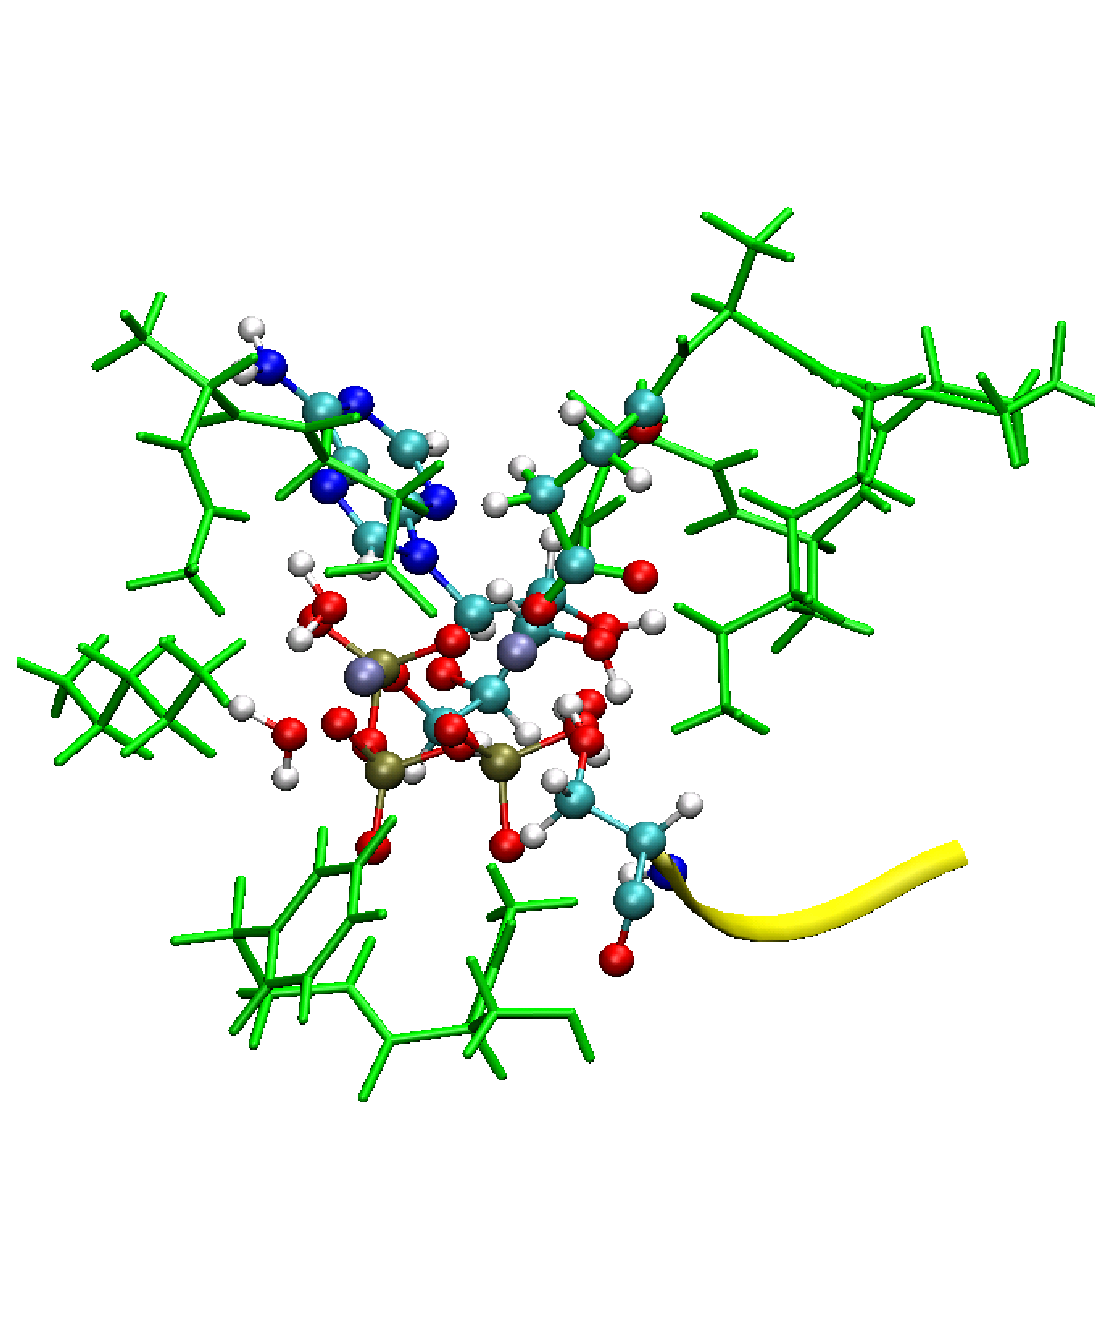
\includegraphics{kinasepicture.ps}}
%\caption{
%The structure of a 263 atom protein kinase A fragment. This structure
%is equivalent to the input structure that has been used
%to test the QUICCA optimizer.}\label{kinasepicture} 
%\end{figure}

\begin{figure}[h]
\resizebox*{3.5in}{!}{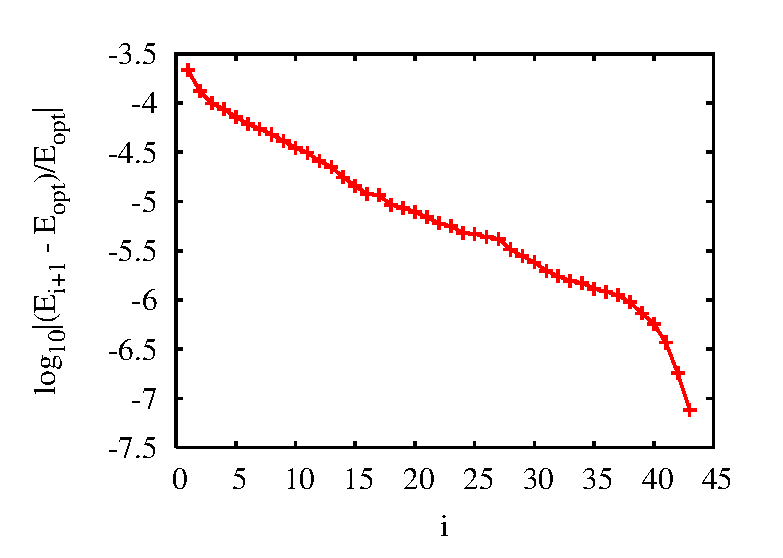
\includegraphics{R263logdata2.eps}}
\caption{
Convergence of the energy with geometry step $i$ on a log$_{10}$-linear  scale for the 
263 atom protein kinase A fragment at the RHF/STO-2G level of theory.}\label{logn-logde} 
\end{figure}

\begin{figure}[h]
\resizebox*{3.5in}{!}{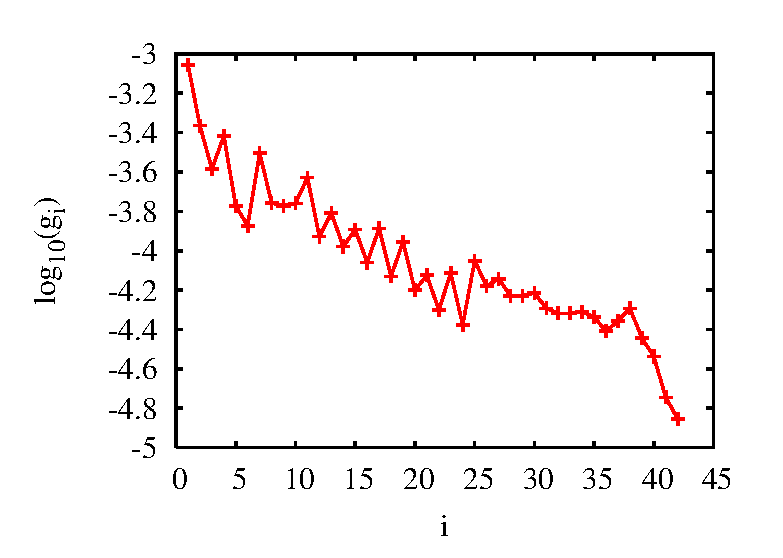
\includegraphics{RMSCartData.eps}}
\caption{
Convergence of the root mean square of the Cartesian gradients, $g_{i}$,
with geometry step $i$ on a log$_{10}$-linear  scale for the 
263 atom protein kinase A fragment at the RHF/STO-2G level of theory.}\label{gradientpicture} 
\end{figure}

\subsection{Convergence}

The simplest possible geometry optimizer, Cartesian steepest descents exhibits linear convergence and can 
be extremely slow for two reasons. One reason is that it cannot cope with 
cases where the condition number of the Hessian is large, 
as for example when floppy modes are present. 
The other reason is the extensive coupling between coordinates.
A comparison between Cartesian and internal coordinate optimizers can be
found in Ref.~\cite{bakerstest}.

In order to briefly compare the performance of different types of optimizers,
it is necessary to review a few important definitions.

%More sophisticated second order methods likewise converge linearly away 
%from the basin of attraction,  but at a more accelerated rate by taking advantage of curvature 
%information to precondition each stepsize.  In the basin of attraction, where the second order approximation 
%to the nonlinear objective is accurate, the Newton-Raphson method achieves second order convergence, 
%while more approximate second order methods (for example quasi-Newton algorithms) can achieve 
%superlinear convergence \cite{RFletcher,Pulay_natural_internals}.   

An optimization algorithm is characterized by the ratio $ {\Delta E_{i+1}}/{\Delta E_{i}^n} =c$,
where $\Delta E_i = |E_{i}-E_{\rm opt}| $ is the absolute error at geometry step $i$,
$E_{\rm opt}$ is the extremal value of the energy, $n$ is the order of convergence, 
and $c$ is the convergence factor \cite{Quarteroni}.  With first order convergence $n=1$, and
the error typically decays exponentially as $\Delta E_i = e^{-f*i}$, where $f=-{\rm log}(c)$ is the 
rate of convergence. 
The case, when $n=1$ and $\lim_{i \to \infty} c = 0$ is called superlinear convergence.

It is important at this point to make the difference clear between the 
rate of convergence for Newton and quasi-Newton methods. 

Newton methods use the exact Hessian and can achive second order 
convergence, i.e. $n=2$, close to convergence.

As far as quasi-Newton methods (e.g. BFGS, DFP, etc. \cite{RFletcher})
are concerned, there is a common 
misunderstanding as if these methods would be assimptotically of second order.
As it has been pointed out by founders of quasi-Newton methods,
these methods achieve maximally superlinear convergence, i.e. they are
of first-order: $n=1$ \cite{RFletcher}. Thus, quasi-Newton methods,
such as those based on Hessian update, like BFGS or DFP, have 
(even assimptotically) only
first order convergence. For an excellent discussion of convergence
properties of quasi-Newton methods see e.g. Chapter 3.2 of Fletcher's book
\cite{RFletcher}.

An earlier work of Fogarasi and Pulay already called the attention 
to this point \cite{Pulay_natural_internals},
but we would like to emphasise it again, as we compare QUICCA to quasi-Newton
methods.

%For large systems and approximate second order methods, the rate of 
%convergence $f$ is the most significant parameter governing efficiency.   Toward convergence,
%approximate second order methods may achieve superlinear convergence, where the rate $f$
%increases  but the order remains $n=1$.  

To investigate the convergence properties of QUICCA in a large application, we have carried out
optimization of a 263 atom fragment of crystallographic Protein Kinase A, involving two Magnesiums, 
ATP and a fragment of the Protein Kinase Inhibitor to which phosphate is transfered. This is a
model reactant system obtained from Ref.~\onlinecite{1ATP} and is shown in 
Fig.~\ref{kinasepicture}.   Optimization was performed at the HF/STO-2G level of theory with an 
approximate energy resolution of $10^{-5}$ Hartrees using MondoSCF \cite{MondoSCF}, with ten peripheral atoms 
constrained to mimic steric effects of the enzyme.  Note that this minimal level of theory actually 
makes more work for the optimizer, as it will tend to move away from the more correct crystallographic 
structure. The number of internal coordinates, generated for this structure
was 1280 at convergence.
Figure~\ref{logn-logde} shows ${\rm log}_{10} \Delta E_i$ vs $i$ for this system, and in 
Fig.~\ref{gradientpicture} the root mean square gradient at each step is shown.   
In Fig.~\ref{logn-logde}, there is a characteristic downturn, indicating
a substantially accelerated convergence and demonstrating superlinear
or maybe even higher order convergence.

%The lines in Fig.~\ref{logn-logde} are a guide to the eye, highlighting change in the rate of 
%convergence $f$;  toward the minimum, the magnitude of $f$ increases substantially, 
%demonstrating superlinear convergence.  

\section{Conclusions}

We have presented a new concept for local optimization, the ``QUasi Independent Curvilinear 
Coordinate Approximation'' or  QUICCA, and applied it to the geometry optimization of molecular 
structures. Achieving super linear convergence and competitive with the most aggressive geometry 
optimizers in the literature, QUICCA has demonstrated that an efficient optimization algorithm 
can be constructed without {\em explicit} coupling in local expansion of the energy.  
However, coupling effects do enter QUICCA {\em implicitly} through a weighted curve fit, 
providing an important averaging effect that compensates for irregularities related
to the independent coordinate approximation.  

The implementation presented here is relatively simple, employing conventional redundant
internal coordinates, a weighted line fit and backtracking, allowing  substantial room for 
improvement.  Indeed, the QUICCA concept opens the door for a wide range of auxiliary techniques 
that may benefit from physical insight (such as the development of more precise weighting schemes) 
as well as from ideas in applied mathematics involving robust estimation, interpolation and 
advanced methods of regression.  

Developed in the context of quantum chemistry, QUICCA is enabling the large scale application of  
linear scaling electronic structure theory to large scale problems in biology and materials science. 
In addition, with the availability of fast linear scaling Cartesian/internal coordinate transforms 
\cite{nemeth_coordtrf1}, the QUICCA algorithm may also present advantages in the optimization of 
large systems employing classical forcefields.

The averaging scheme presented here, achieving an effective decoupled internal coordinate representation
of the potential energy surface, may also be useful in on-the-fly construction of classical force fields.
In such an approach, force field parameters such as the spring-constant and equilibrium position 
would be updated periodically from {\em ab initio} data, taken over several time steps. 
This on-the-fly construction of force fields based on QUICCA might provide a useful  alternative to 
the force matching algorithm of Ercolessi {\it et.al.} \cite{force-matching} and to the reactive 
force field concepts developed by the Goddard group \cite{reaxff1,reaxff2}.

\begin{acknowledgments}
K.~N{\'e}meth gratefully acknowledges {\"{O}}.~Farkas (Budapest) for providing the 
Cartesian coordinates of the Baker's test set, to B.P.~Uberuaga (Los Alamos) for 
calling our attention to Ref.~\cite{force-matching} and to J. {\'A}ngy{\'a}n
(Nancy), S. Lucidi (Rome) and V. Weber (Los Alamos) for discussions.
\end{acknowledgments}

\bibliography{mondo_new}
\end{document}
